\documentclass[tikz,border=2pt]{standalone}
\usepackage{amsmath,amssymb}
\usepackage{tikz}
\usetikzlibrary{arrows.meta}

\begin{document}
% Multiplying a constraint by -1 flips the inequality sign but describes the same half-plane:
% -x_1 + x_2 <= -3 and x_1 - x_2 >= 3 are the same region, now with a nonnegative rhs.
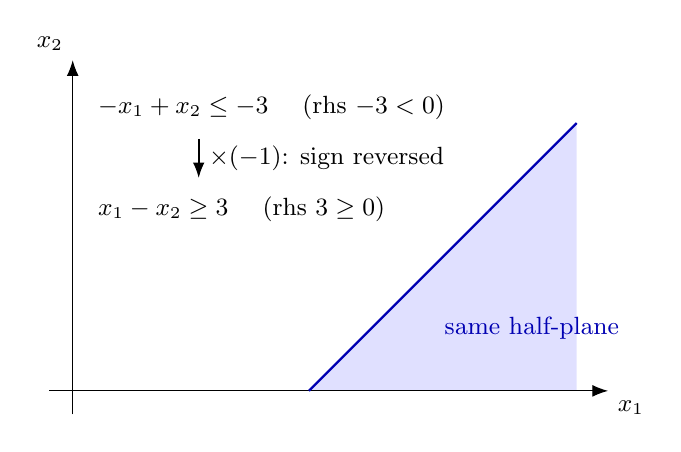
\begin{tikzpicture}[every node/.style={font=\small}, >={Latex[length=2mm]}]
	\fill[blue!12] (3,0) -- (6.4,0) -- (6.4,3.4) -- cycle;
	\draw[->] (-0.3,0) -- (6.8,0) node[below right] {$x_1$};
	\draw[->] (0,-0.3) -- (0,4.2) node[above left] {$x_2$};
	\draw[blue!70!black, thick] (3,0) -- (6.4,3.4);
	\node[blue!70!black, font=\small, anchor=west] at (4.6,0.8) {same half-plane};
	\node[anchor=west, align=left] at (0.2,3.6) {$-x_1+x_2\le-3$ \quad(rhs $-3<0$)};
	\draw[->, thick] (1.6,3.2) -- (1.6,2.7) node[midway, right, font=\small] {$\times(-1)$: sign reversed};
	\node[anchor=west, align=left] at (0.2,2.3) {$x_1-x_2\ge3$ \quad(rhs $3\ge0$)};
	\end{tikzpicture}
\end{document}
